\chapter{Building and Dynamics of the Sexual Contacts Network}\label{ConstruccionYDinamica}

\section{Origin of the Data}

Demographic data from the region of Valencia (Spain) was collected from the Valencian Institute of Statistics (2013)  \cite{IVE}.
Lifetime sexual partners for an individual (LSP) was obtained from the Health and Sexual Habits Survey of 2003 \cite{INE}, and summarized in Table \ref{table1}. 

\begin{table}[H]
\centering
\begin{tabular}{ccccccc}
\toprule
\multicolumn{7}{c}{\textbf{MALES}} \\ \midrule
\textbf{ Age} & \textbf{0 LSP} & \textbf{1 LSP} &\textbf{ 2 LSP} & \textbf{3--4 LSP} & \textbf{5--9 LSP} & \textbf{10 or More LSP} \\
\midrule
14--29 & 0.107 & 0.207 & 0.131 & 0.225 & 0.168 & 0.162 \\
30--39 & 0.027 & 0.225 & 0.128 & 0.21 & 0.17 & 0.24 \\
40--65 & 0.019 & 0.268 & 0.14 & 0.193 & 0.163 & 0.217 \\
 \midrule 
 
\multicolumn{7}{c}{FEMALES} \\ \midrule
  Age & $0$ LSP & $1$ LSP & $2$ LSP & 3--4 LSP & 5--9 LSP & $10$ or more LSP \\
 \midrule
14--29 & 0.138 & 0.43 & 0.186 & 0.158 & 0.056 & 0.032 \\
30--39 & 0.029 & 0.501 & 0.168 & 0.177 & 0.077 & 0.048 \\
40--65 & 0.017 & 0.652 & 0.138 & 0.118 & 0.039 & 0.036 \\
\bottomrule
\end{tabular} 
\caption{Proportion of males and females per number of life sexual partners {LSP} per age group.}
\label{table1} 
\end{table}

Some features of the distribution of contacts were: (i) the percentage of males and females with no partners is
very similar in each age-group; (ii) the proportion of women  with a single partner is, approximately, two times larger than men with only one partner; and (iii) the percentage of men with two or more partners is always larger than that of women except for women in the age-groups 14--29, and~30--39 in the case of two partners. The asymmetry in the behaviour of males and females should be taken into account in the construction of the network.

\section{Network Model}

Before proceeding with the definition of our model, it is convenient to give a brief and general perspective on the emergent field of network research for the readers not familiar with these techniques and their application in epidemiology. A network is, basically, a model which derives from the abstract mathematical concept of a graph composed by a set of points (the so-called nodes) connected among them by some lines or edges (known as ``links'' in the case of networks).

\begin{figure}[ht]
	\centering
	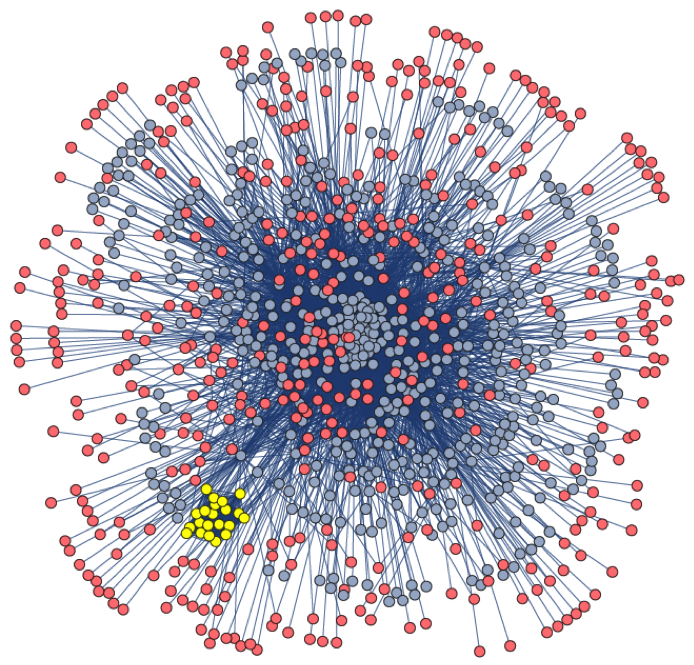
\includegraphics[scale=0.7]{IMG/LSP}
	\caption{Example Network of 1,000 nodes, MSM in yellow, women in red and men in blue.}
	\label{LSPnetwork}
\end{figure}


There are several types of networks of interest for the applied sciences. If we classify them according to the degree of a node, i.e., to the number of links for a given node (or, more properly, to the distribution of these number of links), we have two main categories in the literature: (i) random networks, in which the links or edges occur with a fixed probability and the statistical distribution of this number of links follows a Poisson's law; and (ii) scale-free networks whose distribution of degrees follows a power-law with an
algebraic tail of the form $P(k) \simeq 1/k^\gamma$ with $2 < \gamma < 3$. This means that the nodes with very large degrees are more likely to appear in scale-free networks than those in random networks. Random networks have been used in epidemiology \cite{acedo2011using} and also as an elemetary model of the brain \cite{acedo2013brain}. On the other hand, scale-free networks have been successfully applied to the Internet and biological networks in which some nodes with a very large number of links are determinant in the control of the dynamics (see \cite{dorogovtsev2013evolution}). Small-world networks are also an important paradigm in the science of networks. This concept refers to the average length of a path connecting two typical nodes in the network. It was found that some sparse networks may, on the other hand, present the small-world phenomenon, i.e., we have short paths connecting every pair of nodes through the links with other nodes. A mechanism to generate these networks was discovered by Watts and Strogatz \cite{watts1998collective}. Many networks in sociology exhibit this small-world property \cite{christakis2007spread,liljeros2001web,bearman2004chains}.

In this dissertation, we use the random network model as a basis to simulate the network of sexual contacts among individuals, but, in this model, the average number of connections depend upon the age-group as deduced from Table \ref{table1}. A basic property of the network we are going to discuss is that the total number of lifetime sexual partners (LSP) for the male population (M) must coincide with the total number of LSP for the female population (F). This is so because (in a purely heterosexual network) every link starting on a male must end in a female and viceversa. In mathematical terms:

\begin{equation}
\label{nodeseq}
\displaystyle\sum_{i=1}^M\, LSP_i=\displaystyle\sum_{j=1}^F\, LSP_j\; .
\end{equation}

The estimation of sexual partners: there are some approaches to the number of LSP in males and females \cite{chandra2013sexual,mosher2005sexual} that are difficult to match. Generally speaking, males tend to overestimate the number of their sexual partners and females tend to underestimate it. Therefore, we considered the average LSP male value, $\left\langle k \right\rangle_m$, and calibrated the network so that results were consistent with data of Table \ref{table1}, and estimated that the number of LSP in males in Spain was at least $4.5$. Networks with 250,000, 500,000 and 750,000 have been necessary to perform the present study. It required a substantial computational power.

\section{Semi-Random Construction}
\label{subsec22}

From Table \ref{table1} (proportion of male LSP aged 14--29), we have the following list:
$( 0.107, 0.314, 0.445, 0.67, 0.838, 1)$ for the accumulated proportion of males less than or equal to a given LSP number.
Now, we randomly generate a number $r$ between $0$ and $1$ and assign the number of contacts to every male node in the $14-29$
age group, in the network as follows:

\begin{itemize}[leftmargin=*,labelsep=5mm]
\item $r \le 0.107$ say that the corresponding male does not have an LSP,
\item $0.107 < r \le 0.314$ say that the corresponding male has one LSP,
\item $0.314 < r \le 0.445$ say that the corresponding male has two LSPs,
\item $0.445 < r \le 0.67$  say that the corresponding male has three or four LSPs uniformly distributed.
\item $0.67 < r \le < 0.838$ say that the corresponding male has five to nine LSPs uniformly distributed.
\item $0.838 < r \le 1$ say that the corresponding male has 10 or more LSPs.
\end{itemize}

Every node in the network is labelled by its gender and age randomly assigned according to the population histogram. The assignment of the number of bonds, as another label of the node, is not so straightforward since we must guarantee that the condition in Equation\ (\ref{nodeseq}) is verified. In~order to fulfill this condition, we take advantage of the uncertainty of statistics reports concerning individuals with $10$ or more LSPs.
%ANSWER: "Lifetime sexual partners" as been replaced by LSPs.
Starting with the males, we assign the number of LSPs up to nine partners and, for $10$ or more partners proceed as follows: let $i_{\mbox{max}}$ be the number of males with nine or less partners. The unassigned males should be $M-i_{\mbox{max}}$ and the number of bonds that should be distributed among them is $M \left\langle k \right\rangle_m-\sum_{i=1}^{i_{\mbox{max}}}\, LSP_i$. By Euclidian division, this quantity can be expressed as $(M-i_{\mbox{max}}) n_m+r_m$, where $n_m \ge 10$. In our procedure, we assign a random number of bonds, uniformly distributed, in the interval $\left[10,2 n_m-10\right]$ to every male with $10$ or more LSPs, i.e.,
to~the $M-i_{\mbox{max}}$ unassigned males.

Now, we denote as $p_m$ the total number of bonds of the male population. We must take into account, as expressed in Equation\
(\ref{nodeseq}), that the total number of bonds of the female population should be the same. To impose that condition, we
proceed as follows: (i) assign the number of bonds to the females with nine or less partners following the statistical 
data in Table \ref{table1}; and (ii) the sum of all female LSPs in this group of $j_{\mbox{max}}$ members will be denoted by $s_f$. 
Then, $n_f=F-j_{\mbox{max}}$ is the number of females with $10$ or more LSPs; and (iii) the number of bonds starting in the males and still unassigned to a female is $p_m-s_f= q_f n_f + r_f$, where $0 \le r_f < n_f$ and $n_f \ge 10$. (iv) We assign $q_f+1$ bonds to $r_f$ females still unassigned and $q_f$ bonds to the rest of $n_f-r_f$ females. The steps of this algorithm are also enumerated in the flow diagram in Figure  \ref{flux1}.

Notice that, for men and women with more than 10 LSPs, we assign their LSP in the most equitable way, assuming that all of them have, more or less, the same number of LSPs. Thus, we have a lot of hubs with a low number of contacts instead of a few hubs with a lot of contacts.

From the point of view of STI transmission, the latter situation leads to a faster transmission if the hub is infected, and, also, if the hub is vaccinated, the transmission is cut faster. Therefore, due to the lack of data about people with $10$ or more LSPs, we make the decision of being conservative in the transmission of the disease and in the effect of the vaccination campaigns.

Notice that this procedure implies that the condition in Equation\ (\ref{nodeseq}) is verified. After this procedure, we have obtained the following lists:
\begin{itemize}[leftmargin=*,labelsep=5mm]
\item $AgeMale\left[ i \right]$ is the age of the i-th male, $i=1,\ldots,M$,
\item $AgeFemale\left[ i\right]$ is the age of the i-th female, $i=1,\ldots,F$,
\item $kMale\left[ i \right]$ is the number of LSP for the i-th male, $i=1,\ldots,M$,
\item $kFemale\left[ i \right]$ is the number of LSP for the i-th female, $i=1,\ldots,F$.
%ANSWER: “lifetime sexual partners” has been replaced by “LSP” 
\end{itemize}

\begin{figure}[H]
\centering
\begin{tabular}{c}
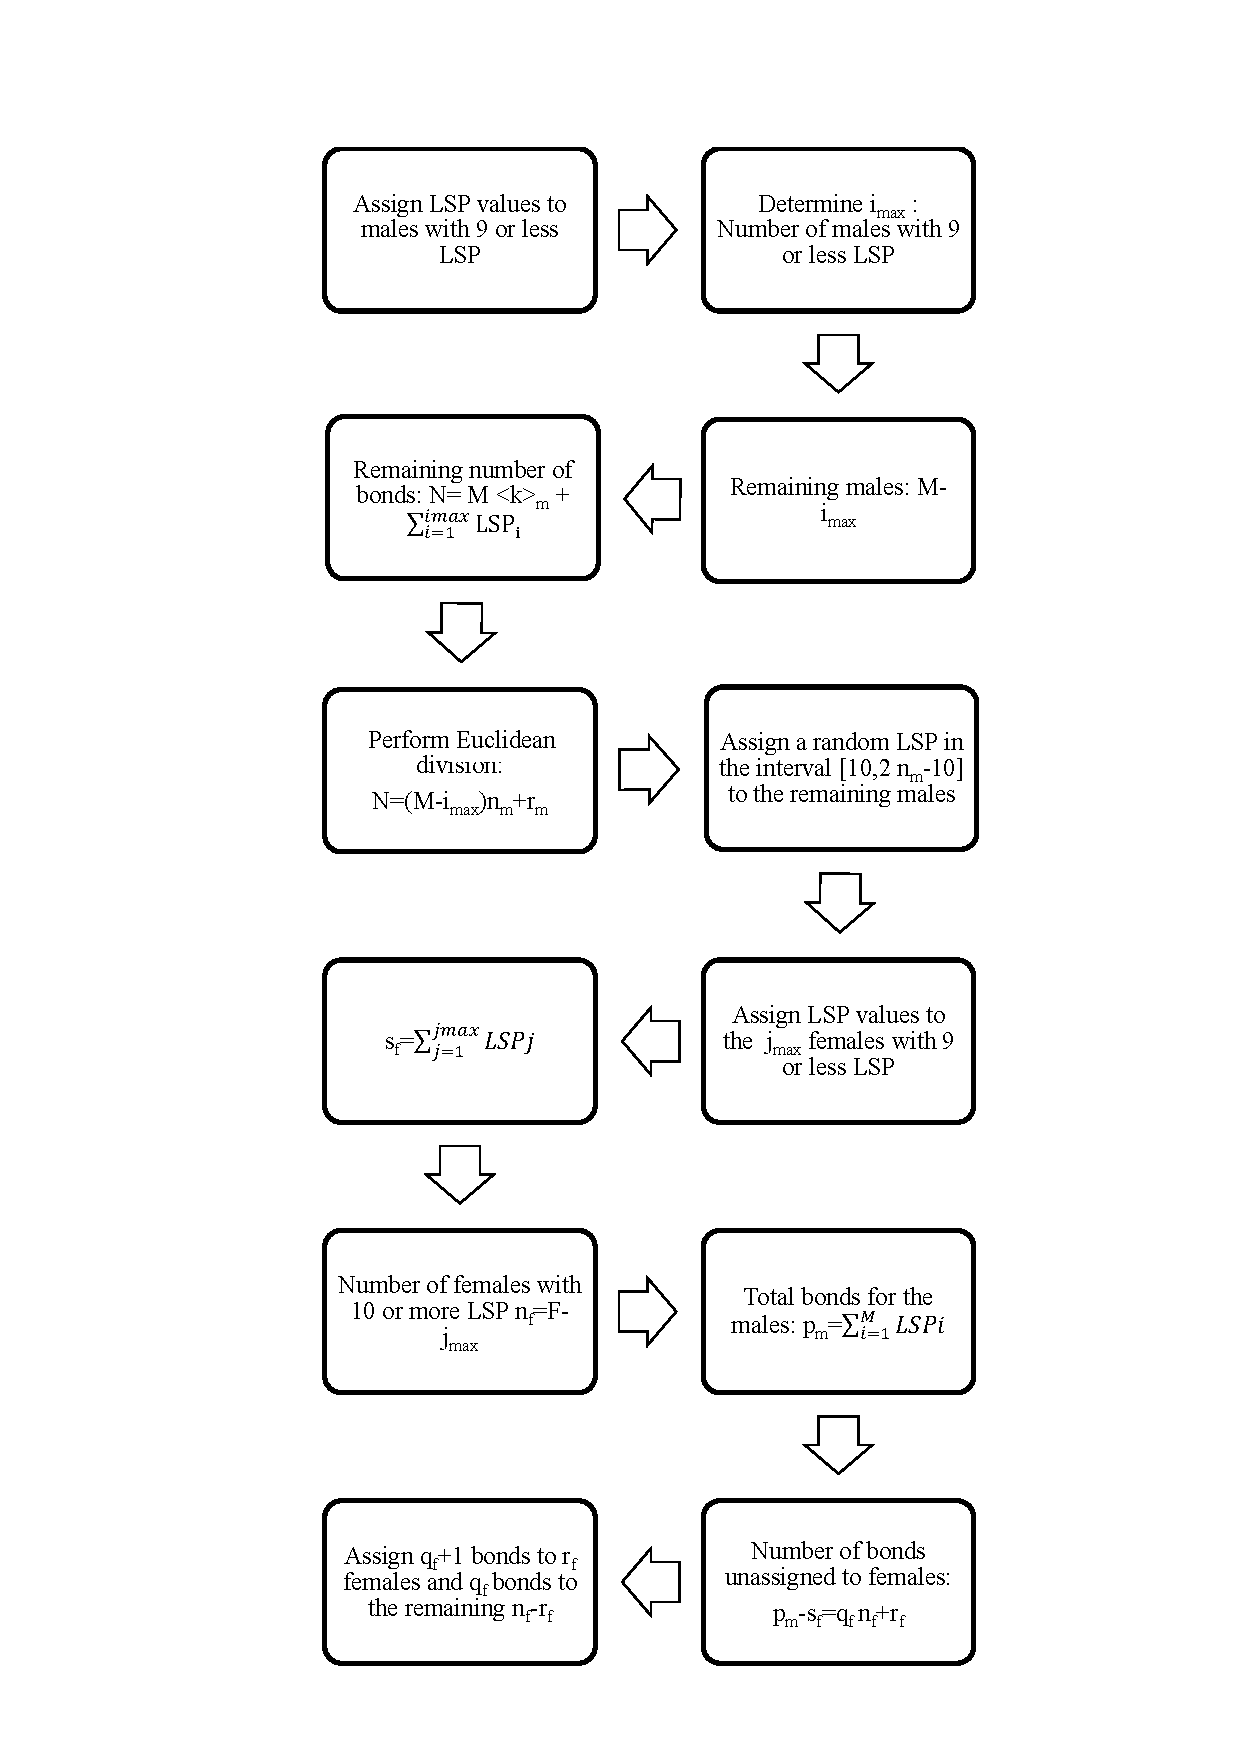
\includegraphics[width=\textwidth]{IMG/FluxDiagramI.pdf}
\end{tabular}
\caption{Flow diagram for the algorithm corresponding to the assignment of a number of LSPs to every male and female in the network.\label{flux1}}
\end{figure}

These lists will be used to perform the connections of males and females and build the network.
Note that, in Table \ref{table1}, there are more females than males with few LSPs (comparing male and female percentages). It implies that there will be few women with a very large number of LSPs. This fact suggests us to start the assignment procedure with women with the largest LSPs. Otherwise, it would be possible that, when we have to assign LSPs of men to a female with a large number of LSPs, there~will not be enough men with free sexual partners to be assigned and, for this female, it would be impossible to satisfy the condition that the degree of each node was the number of its LSP. 

The assignment of partners was carried out by considering a principle of psychological similarity~\cite{gentner1997structure} or assortativity.
Hence, we are going to define a weight function assuming that: women with few LSPs usually match men with few LSPs; people with four or more LSPs use to join with people with four or more LSPs; and couples where one of them has a large number of LSPs and the other few LSPs will be uncommon. Then, for the woman $i$ and the man $j$, we define the following weight~function:

\begin{equation}
\pi(i,j) = 
\begin{array}{l}
\left\lbrace \begin{array}{lc}
| kFemale[i] - kMale[j] | & kFemale[i], kMale[j] \le 4 \\
0 & kFemale[i], kMale[j] > 4 \\
100 & \mbox{otherwise}
\end{array} \right\rbrace, \\
\\
 + | AgeFemale[i] - AgeMale[j] - 1.8 |.
\end{array}
\label{peso}
\end{equation}

The combined weight function, which takes into account the age difference of the partners, $\vert AgeFemale[i] - AgeMale[j] - 1.8 \vert$ is defined in this way because some studies show that the average age difference among the members of a couple in Spain is $1.8$ years \cite{miret2010similitud}. 

The MSM population (around a $3.88$ \% of the total male population in Spain) can also be incorporated into the model, but, in this subpopulation, the connectivity would be larger than the heterosexual network.
The MSM population would also be connected with the heterosexual one by links with women in such a way that every MSM individual has a link with a woman with five or more contacts \cite{acedo2017calibrating}. The assignment of links is then performed by the a Greedy Randomized Adaptive Search Procedure (GRASP) algorithm 
%Pls define. 
%ANSWER: Done.
\cite{cormen2009introduction,feo1995greedy}. Details~about the construction of the whole network have been provided in previous studies \cite{acedo2017calibrating,BuildingLSPNova}. 

\section{The Dynamics of HPV Transmission in the Sexual Network}

To implement the simulation of the transmission of HPV among the individuals in the network, a~standard epidemiological model with susceptible and infected states and three types of infections (HR, LR and co-infection) was carried out.
%please define
%ANSWER: It has been defined in the 1st paragraph of the Introduction. If you consider to recall it again, it can be included as follows ".. infections of high risk (HR), low risk (LR) and co-infection ...". 
The epidemiological model is defined by the following parameters:

\begin{itemize}[leftmargin=*,labelsep=5mm]
\item We need some probabilities to determine if a sexual partner is going to produce a contagion of another partner in a given time stage. These parameters are different for each age group:	
 14--17, 18--29, 30--39 and 40--65. Notice that this means that the probability of contagion depends upon the age group of the members of the relationship. Moreover, the probability of connection of these members in the network is also age-dependent
as proposed in Equation (\ref{peso}). The values of these probabilities are determined in the process of the model fitting.
%ANSWER: Change "fitting of simulations" by "model fitting".
\item Average time an individual infected by a HR HPV clears the infection and recovers.
\item A similar parameter for clearing the LR HPV infection.
\item If a partner produces the contagion of his/her partner, we need another four parameters to determine if the high or low risk HPV infection is transmitted from man to woman and vice versa. 
\end{itemize}

Another additional parameter is necessary to generate the network. This is the average number of LSPs for men (parameter $k$). Simulations are run by generating a network and carrying out a large number of epidemic evolution time-steps starting with a number of individuals infected by both HPV types as given by the CLEOPATRE study \cite{castellsague2012prevalence}.
After the warm-up period, we obtain a stable situation and we can proceed with the calibration by comparing the model predictions with real data and deducing the most probable values of the set of parameters.

We have used a calibration procedure using the Particle Swarm Optimization (PSO) algorithm. The prevalence data for each age group is listed in Table \ref{datosConstruccion}:

\begin{table}[H]
	\centering
	\caption{Prevalence of HR- and LR-infected women per age groups from the 
%Pls define
%ANSWER:It has been defined in the 1st paragraph of the Introduction. Also, it appears in the list of the abbreviations.	
CLEOPATRE study \protect\cite{castellsague2012prevalence}. Co-infections are included in both HR- and LR-infected, mean and $95\%$ confidence intervals.}
	\begin{tabular}{cccc}
		\toprule
		\textbf{Women} & \textbf{HR-Infected} & \textbf{LR-Infected} \\
		\midrule
		18--29 y.o. & $24.10\%,$ $[21.33\%, 26.98\%]$ & $6.36\%,$ $[4.71\%, 8.07\%]$ \\
		30--39 y.o. & $11.01\%,$ $[7.54\%, 15.09\%]$ & $1.26\%,$ $[0.0\%, 3.14\%]$ \\
		40--64 y.o. & $5.96\%,$ $[4.29\%, 7.8\%]$ & $2.37\%,$ $[1.22\%, 3.68\%]$ \\
		\midrule
		18--64 y.o. & $16.23\%,$$[14.52\%, 17.97\%]$ & $4.41\%,$ $[3.42\%, 5.45\%]$ \\
		\bottomrule
	\end{tabular}
	\label{datosConstruccion}
\end{table}

Note that the network building and the transmission parameters involve randomness and uncertainty due to the random processes used in the network building and the transmission dynamics of the HPV. This fact is going to be taken into account in the  calibration and simulation.

Due to the randomness of the simulations, we will show the average and confidence intervals among the $30$ simulations per every scenario that we have considered above. This number was chosen as a compromise among efficiency of the method and computational feasibility. We have found that, with these runs, we obtain reasonable parameters in many of the simulations. Of course, it would be useful to increase this number, but this cannot be achieved, in a sensible computing time, with the computational resources that we devoted to the task. For example, a single run takes $162$ hours per run for a network of $500,000$ nodes and $256$ hours in the case of $750,000$ nodes (in a single processor of a Sandy Bridge platform). Simulations were run on a multi core platform with $64$ processors and $500$ GB RAM and every processor was assigned with the computation of a simulation for a given set of parameters.

%\section{Calculation of the Number of Infections} Comentario en rojo de Rafa%
\section{Decline of infections}

We call $I$ the number of infected women of LR HPV 6 and/or 11 just before the starting of the vaccination campaign; we call $V = ( v_1, \ldots, v_N)$ to the number of infected women of LR HPV 6 and/or 11 every month from the starting of the vaccination program until the end of the simulation. Then,~the~vector 

\begin{equation}
100 \times \left( 1-\displaystyle\frac{v_1}{I}, \ldots, 1-\displaystyle\frac{v_N}{I} \right) \; 
\end{equation}
is a measure of the percentage of decline of number of infected women of LR HPV 6 and/or 11 after the beginning of the vaccination campaign. This will also be applied to men and MSM.

In order to compare GW data given in \cite{ali2013genital} with our model, results referred to infected women of LR HPV 6 and/or 11, we should take into account that, whether a fixed proportion of HPV 6 and/or 11 infected individuals develops warts, the percentage of decline in warts and in infected women of LR HPV 6 and/or 11 will be comparable. 

Another important issue for the natural history of the disease is the persistence of the infection \cite{campos2014updated}. Our model does not consider the persistence ``a priori'', but we derive the cases of genital warts from the number of cases of infected individuals by taking this data into account.
